\section{Philosophie}

\begin{center}
\begin{tabular}{|c l|}
\hline
\rowcolor{red!10}\textbf{Règle 2.1} & Garder à tout instant à l'esprit la philosophie \og KISS  : Keep It Smart and Simple \fg{}. \\
\rowcolor{red!10} & \quad trad. \og  Garde Cela Simple et Malin \fg{} \\ \hline
 & Garder le code simple, fonctionnel et si possible élégant. Il est important que d'autres \\
 & développeur du groupe puisse facilement comprendre le rôle d'une section de code et les \\
 & actions qu'il effectue. Dans cette optique, il est également important que le code ne \\
 & soit pas plus complexe que nécessaire (à ce titre voir \textbf{Règle 2.2}). \\ \hline
\hline
\end{tabular}
\end{center}

\smallskip
\begin{large}
\textbf{\textsc{Remarque :}}
\end{large}
De façon plus particulière, il ne faut jamais supposer que le code, aussi clairement rédigé soit-il, documente de façon suffisante par lui même le comportement attendu à l'exécution. Dans cette optique, il est d'importance capitale de commenter et de documenter toute partie du code qui ne serait pas triviale pour un néophyte. (voir \textbf{Figure \ref{self-documented-code} Page \pageref{self-documented-code}} pour une illustration humoristique)
\begin{figure}\centering
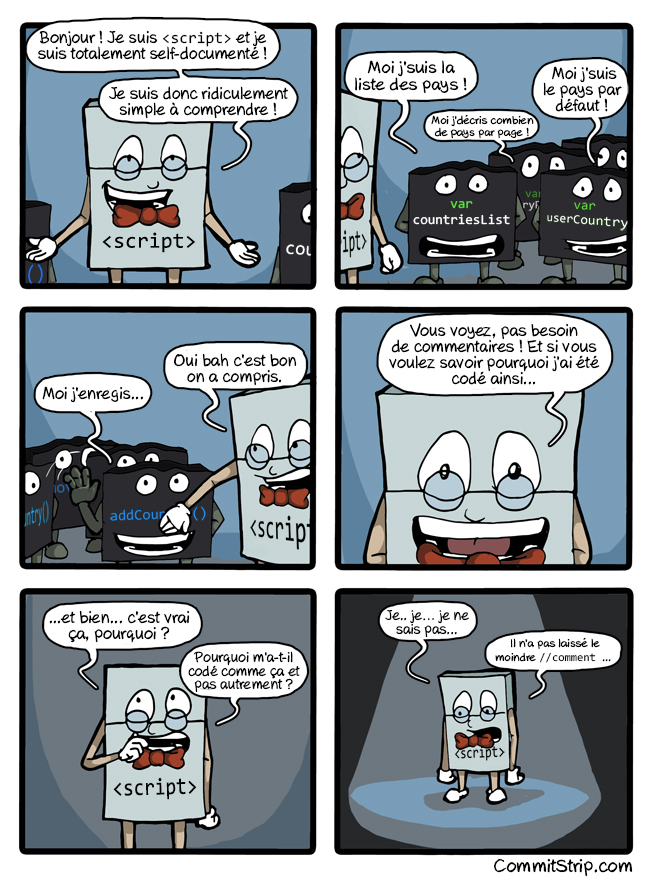
\includegraphics[scale=0.6]{pictures/CommitStrip_self-documented.jpg}
\caption{Code auto-documenté}
\label{self-documented-code}
\end{figure}

\medskip

\begin{center}
\begin{tabular}{|c l|}
\hline
\rowcolor{red!10}\textbf{Règle 2.2} & \og You Ain't Gonna Need It \fg{} est également un principe de base. \\
\rowcolor{red!10} & \quad trad. \og  Tu n'en Auras Pas Besoin \fg{} \\ \hline
 & Il est nécessaire de ne coder que ce qui répond à un besoin à un instant donné. Tout \\
 & code rédigé « en prévision de » constitue une perte de temps dans la réalisation de la \\
 & tache en cours et ne rendra l'ensemble du code écrit que plus complexe à valider et \\
 & seras potentiellement source de bugs. \\ \hline
\hline
\end{tabular}
\end{center}

\medskip

\begin{center}
\begin{tabular}{|c l|}
\hline
\rowcolor{red!10}\textbf{Règle 2.3} & Il ne doit pas y avoir de code inatteignable au sein d'un même projet. \\ \hline
 & Une section de code inatteignable est une section de code inutile ou désuète dans le \\
 & contexte où elle est identifiée. Conserver une section de code inatteignable alourdi \\
 & inutilement le code. \\ \hline
\hline
\end{tabular}
\end{center}

\smallskip
\begin{large}
\textbf{\textsc{Exception :}}
\end{large}
On pourra utiliser des drapeaux de compilation afin de gérer l'activation de fonctionnalités dans des sections de codes communes à plusieurs projets. Cela doit être documenté clairement.

\medskip

\begin{center}
\begin{tabular}{|c l|}
\hline
\rowcolor{red!10}\textbf{Règle 2.4} & Le code mis en commentaire est interdit. \\ \hline
 & Le code mis en commentaire constitue une pollution visuelle pour le programmeur et peut \\
 & potentiellement l'induire en erreur en lui proposant d'effectuer une action qui peut \\
 & s'avérer au mieux non nécessaire et au pire potentiellement dangereuse. \\ \hline
\hline
\end{tabular}
\end{center}

\smallskip
\begin{large}
\textbf{\textsc{Exception :}}
\end{large}
Dans un bloc de commentaire descriptif, on pourra faire figurer du code d'exemple, clairement documenté comme tel.


\pagebreak

